\chapter{Muon Generation Processes} \label{sec:generation}

Regarding the natural generation processes, muons with energies above a GeV detected at the surface are produced by cosmic-ray or neutrino interactions.
While muons with these energies can still be produced at particle physic experiments, at energies above several TeV, even the strongest accelerator experiment, the LHC, is not powerful enough to create such energetic muons.
Those high energetic muons can only be created by cosmic-rays or neutrinos.

At the Earth's surface, most of the muons are going downward, originating from interactions of cosmic-ray in the atmosphere.
After $\mathcal{O}(\num{e4})$ meter-water-equivalent (mwe) even the highest energetic muons lost all of their energy and stop before they decay \cite{PDG20}.
Therefore all muons propagating longer distances through the Earth will get absorbed.
Only neutrinos can travel through the Earth without any interaction and can convert to their charged leptonic counterpart just before the surface.
Therefore muons seen in a detector going downward most-often originate from cosmic-rays while upward-going muons originate from neutrino interactions.

\section{Cosmic-Ray induced Muons}

Cosmic-rays hit the atmosphere with a rate of \SI{1}{kHz/m^2} and consist mainly of Protons (\SI{75}{\percent}), Helium (\SI{17}{\percent}) and heavier nuclei \cite{Gaisser16CR}.
Depending on the energy range these ratios are shifted towards the heavier nuclei, mainly iron, dominating at higher energies.
The cosmic-ray spectrum is shown in \figref{fig:cosmic_rays} together with models describing the composition of the nuclei.

\begin{figure}
    \centering
    \begin{subfigure}{0.9\textwidth}
        \centering
        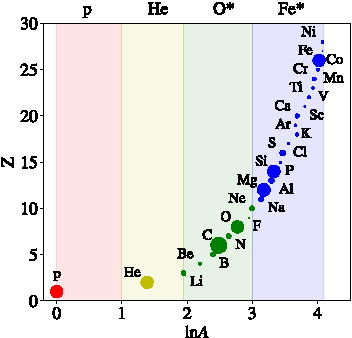
\includegraphics[width=0.5\textwidth]{./images/cosmic_ray_composition.pdf}
        \caption{Composition of the cosmic-rays grouped nearly equally in their logarithmic mass between proton and nickel. The size of the circles denotes the flux ratio compared to the leading element in each group. \cite{Dembinski17GSF}}
        \label{fig:cr_components}
        \vspace{0.5cm}
    \end{subfigure}
    \begin{subfigure}{0.9\textwidth}
        \centering
        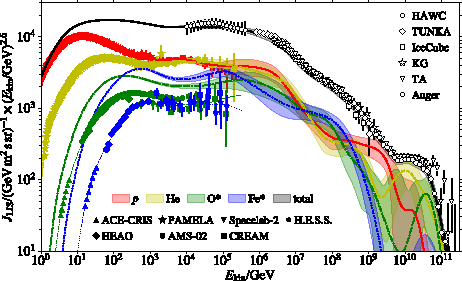
\includegraphics[width=\textwidth]{./images/cosmic_ray_spectrum.pdf}
        \caption{Global Spline Fit of the measured all-particle cosmic-ray energy spectrum. For Oxygen and Iron the data points represent the measured elemental flux and the model lines are shown without error bars for the elemental flux and with error bars for the group flux. \cite{Dembinski19MuonPuzzle}}
        \label{fig:cr_spectrum}
    \end{subfigure}
    \caption{The energy spectrum of the cosmic-rays from the GeV range to the GZK-cutoff. Up to a PeV, space-based detectors measure the cosmic-rays directly being able to differentiate between the compositions. Above a PeV, ground-based detectors measure the cosmic-rays indirectly via air showers.}
    \label{fig:cosmic_rays}
\end{figure}

\subsection{Cosmic-Ray Energy Spectrum}

The energy spectrum of incoming cosmic-rays, shown in \figref{fig:cr_spectrum}, is focusing above the GeV energy range where most of the particles are produced outside of our solar system.
Until energies of roughly a GeV the main source of measured cosmic-ray events originates from our sun with a variable event rate depending on the sun's activity.
Cosmic-rays from outside of our solar system are screened by the Heliosphere.

Above a GeV, the magnetic fields of the sun are not powerful enough to accelerate particles to such high energies and galactic sources are the main source of cosmic rays.
The main type of cosmic accelerators is considered supernova remnants (SNRs).
Supernov\ae{} occur on average once in a century in our galaxy, while their shock waves propagate hundreds of years into the interstellar medium.
The particles with these energies are considered to undergo the so-called Fermi acceleration, a shock acceleration resulting in a power-law spectrum $E^{-\gamma}$ with an index of $\gamma = \num{2}$.
Due to interaction losses and the probability to escape the galactic magnetic field the spectrum gets steeper and results in a measured spectral index of \num{2.7} on Earth.
SNRs can accelerate particles up to a PeV, a region called the \textit{knee} of the spectrum.

Above the \textit{knee} and until the so-called \textit{ankle} at an EeV yet unknown galactic sources, probably Pulsars or Quasars become dominant resulting in an increased measured spectral index of \num{3.1}.
Above the \textit{ankle} sources inside our galaxy are not powerful enough to accelerate such high energetic particles and extragalactic sources, e.g. Active Galactic Nuclei, become the main contributor.
The resulting spectral shape flattens again to an index of \num{2.6}.
At around \SI{1e20}{eV} the protons interact with the photons of the CMB to a Delta resonance, resulting in the GZK-cutoff of the energy spectrum, predicted by Greisen, Zatsepin and Kuz'man \cite{Greisen66GZK, Zatsepin66GZK}.

\subsection{Cosmic-Ray induced Air Shower} \label{sec:air_shower}

When cosmic-rays reach the Earth they interact with the dense medium of the atmosphere.
Depending on the energy and the composition of the particle, the height of the first interaction is at \SIrange{10}{15}{km}.
The secondary particles of this interaction again interact with the atmosphere resulting in a particle cascade or air shower that consists of thousands or even billions of particles.
These showers can be categorized into hadronic, muonic and electromagnetic shower components, which are illustrated in \figref{fig:air_shower_components}.

\begin{figure}
    \centering
    \begin{subfigure}[t]{0.47\textwidth}
        \centering
        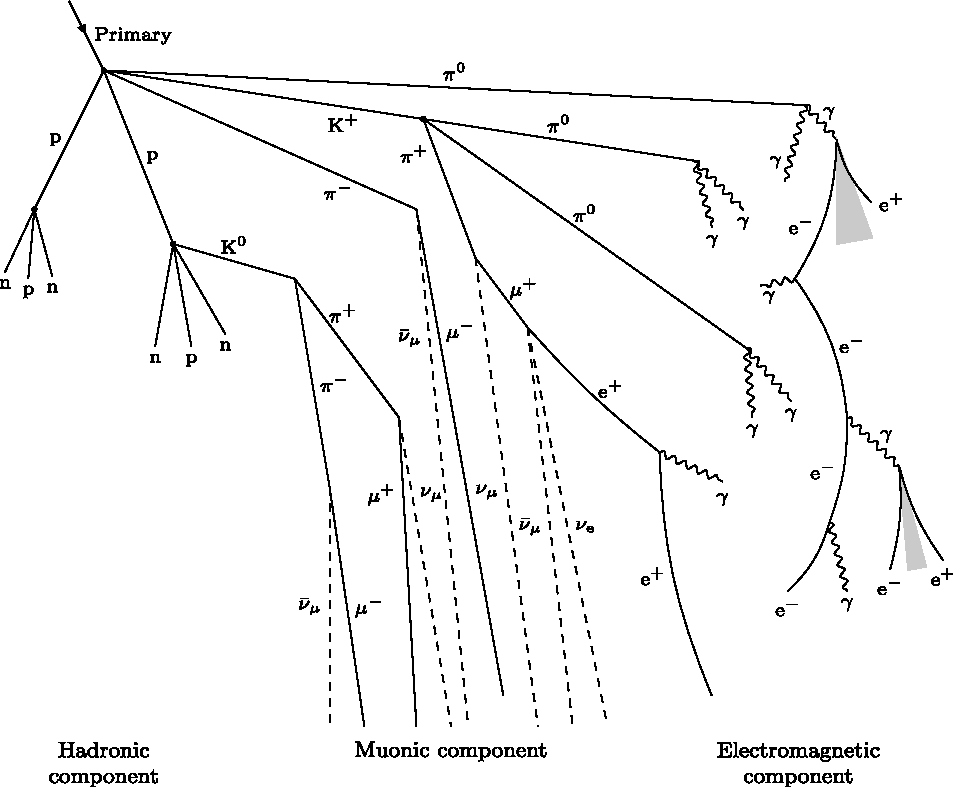
\includegraphics[width=\textwidth]{./images/air_shower_components.pdf}
        \caption{Basic scheme of the interactions and particles for the shower components of an air shower. \cite{Barrantes18EAS}}
        \label{fig:air_shower_components}
    \end{subfigure}
    \hfill
    \begin{subfigure}[t]{0.47\textwidth}
        \centering
        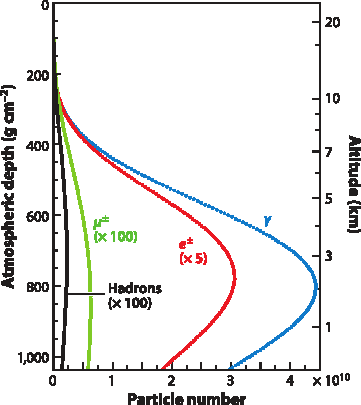
\includegraphics[width=\textwidth]{./images/air_shower_development.pdf}
        \caption{Development of the number of produced shower particles for a \SI{e19}{eV} proton induced vertical air shower. \cite{Engel11EAS}}
        \label{fig:air_shower_development}
    \end{subfigure}
    \caption{Development of a cosmic-ray induced air shower. To the left the different sub-showers divided into an electromagnetic, a muonic and a hadronic component is shown. To the right the contribution of these sub-showers and particles during the shower development is shown.}
    \label{fig:air_shower}
\end{figure}

\textbf{The electromagnetic shower component} consists of electrons, positrons and photons.
Starting e.g. with a high energy photon the two main gamma interactions are the production of an electron-positron pair, also called the Bethe-Heitler process, and Compton Scattering.
While the latter is just important for the deflection, the pair production is the important process for the shower development.
The produced electrons and positrons dominantly lose their energy via bremsstrahlung, creating again a high energy photon.
The Positron can also annihilate with the atomic electrons creating a photon pair, which is a sub-dominant process.

(TODO: wie viel Energie geht in einem cyclus verloren? vgl Tau-Regeneration)
The cycle of photon pair production and electron/positron bremsstrahlung continues until the bremsstrahlung photons are below an MeV and therefore not energetic enough to create an electron/positron pair.
Due to the high number of charged particles (c.f. \figref{fig:air_shower_development}) that are created, this shower component produces the dominant amount of the Cherenkov light and is also important for the radio signal of a shower.
The production of a muon pair is a sub-dominant process as the muon mass is 200 times higher than the electron mass decreasing the phase space and is therefore not important for the electromagnetic shower development.
However, it is a non-negligible process regarding the number of produced muons inside the shower, while the main production originates from the hadronic shower.

\textbf{The hadronic shower component} mainly consists of the lightest mesons, charged Pions and Kaons ($m_{\pi^{\pm}} \approx \SI{140}{MeV}, m_{K^{\pm}} \approx \SI{494}{MeV}$ \cite{PDG20}).
Due to their relatively long lifetimes of $\tau_{\pi^{\pm}} = \SI{26}{ns}$ and $\tau_{K^{\pm}} = \SI{12}{ns}$, they propagate and lose a significant amount of their energy through interactions before they decay.
Pions decay mainly into muons, as their rest mass is just slightly higher.
Kaons either directly decay into muons (or electrons) or first decay into Pions, which then decay to muons and neutrinos.
The energy losses during the propagation of the Pions and Kaons lead to a steepening of the resulting muon and neutrino energy spectrum to a spectral index of \num{3.7}.
The muons or neutrinos originating from these processes are called \textit{conventional atmospheric} muons or neutrinos.

In addition to Pions and Kaons also short-lived mesons and baryons are produced in hadronic showers.
They consist mainly of mesons with a charm quark, like the D-Meson, of $\Lambda$-Baryons and unflavored mesons, while the latter do not often decay into muons and muon neutrinos.
Due to their short lifetime ($\tau \leq \SI{1}{ps}$), they do not lose energy during their short propagation and directly decay.
The resulting energy spectrum of the decay products is therefore similar to the primary spectrum as the spectral index does not change.
Although these processes are sub-dominant, the flatter spectral index of the resulting muons and neutrinos makes them relevant at higher energies.
Due to the direct decay of the hadrons, which mainly consist of charmed mesons, the resulting muons or neutrinos are called \textit{charmed} or \textit{prompt atmospheric} muons or neutrinos.

\textbf{The muonic shower component} mainly originates from the hadronic shower component and produces just a few secondaries compared to the other shower particles.
The high muon mass ratio compared to the electron also decreases the interaction probability as the bremsstrahlung cross section is proportional to $1/m^2$.
Combined with the relatively high lifetime, the muon range through dense media is the highest, neglecting neutrinos, making them the biggest background for all particle detectors even if they are located deep underground.
Except for detectors placed at high altitudes, they are the only shower component for inclined showers measured on the Earth's surface, neglecting the electromagnetic radiation like Cherenkov light, Fluorescence light or the radio signal.
The resulting muon and neutrino energy flux from cosmic-ray induced air showers is shown in \figref{fig:atmo_mu_nu_flux}.
\begin{figure}
    \centering
    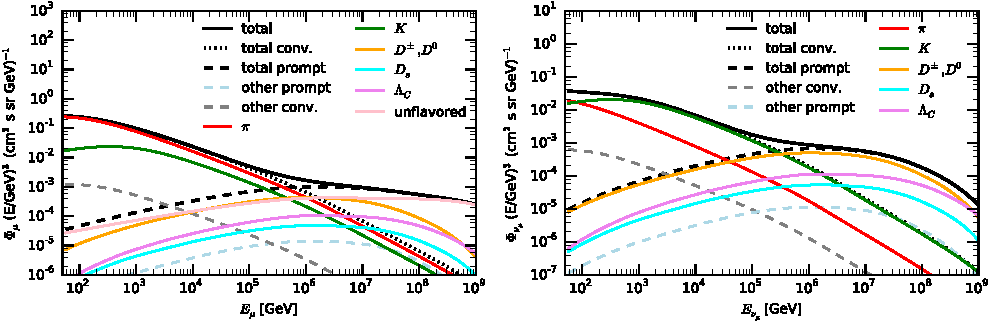
\includegraphics[width=\textwidth]{./images/mceq_mu_nu_flux.pdf}
    \caption{Predictions of the atmospheric muon and neutrino flux at the surface using matrix cascade equations. \cite{Fedynitch15MCEq}}
    \label{fig:atmo_mu_nu_flux}
\end{figure}

A longitudinal shower profile and the contribution of the different sub-shower types is shown in \figref{fig:air_shower_development}.
An increasing number of particles at the beginning of the shower development can be seen as well as a decreasing part when more and more bremsstrahlung photons are too low energetic to produce an electron-positron pair.
The resulting maximum of the longitudinal shower profile $X_{\mathrm{max}}$ at roughly \SI{5}{km} for vertical showers varies for the different primary particle types and energies making it an important feature to classify the primary particle.

Another important feature to estimate the energy of the primary particle is the number of muons detected at the Earth's surface.
Unfortunately, there is a discrepancy between the number of muons measured in air shower detectors, which exceeds the number of muons produced in air shower simulations starting at primary energies of \SI{e16}{eV} \cite{Dembinski19MuonPuzzle}.
That is seen across multiple experiments with a significance of \SI{8}{\sigma}, known as the \textit{Muon Puzzle}.

It is considered, that most of the discrepancy arises from the uncertainties of the hadronic interaction models.
While most of the models are influenced by accelerator measurements from e.g. the LHC, these models provide good agreements for high transversal momentums.
In the forward direction, the beam pipe and not a detector is located, which is fine for those experiments as most differential cross sections diverge in the forward direction.
However, astroparticle physics experiments most often measure the shower in the forward direction leading to fewer cross-checks with the accelerator measurements.
This type of challenge to evaluate cross section also in the forward direction does not just occur for the hadronic models, but for all types of particle interaction including the muon cross sections.

A precise description of the muon bundles is also crucial for underground detectors to separate these background events from their signal.
While there are also muons with a high transversal momentum compared to the shower axis resulting in a lateral distribution for the \SI{e19}{eV} event in \figref{fig:air_shower_muon_surface} of kilometers \cite{Engel11EAS} most of the high energetic muons propagate close to the primary direction making a separation between them challenging.
An extraction of muon physics parameters out of these muon bundles is therefore limited and single muons are required to provide a deeper understanding.

TODO: Plot showing the simulated muon arrival distribution of an air shower on the Earths surface. Ask DBaack

%
% 
% small seperation between the chapters
%
%

\section{Neutrino induced Muons}

Compared to the cosmic-ray induced muons that occur only in bundles, neutrinos produce single muons.
Further muons are produced in the hadronic cascade at the neutrino vertex or as muon pair production.
But these muons have much less energy and stop far before the main muon produced by the neutrino, so they can be neglected regarding muon energies of GeV or above.

\subsection{Neutrino Energy Spectrum}

The neutrino energy spectrum shown in \figref{fig:neutrino_spectrum} is assumed to starts with a high number of cosmological neutrinos or the cosmic neutrino background (C$\nu$B).
Like the CMB they are left-overs from the big bang when the temperature drops below the critical value of weak lepton production and annihilation.
It consists of all neutrino flavors but the energies are far too low to be measurable with current technology.
\begin{figure}
    \centering
    \includegraphics[width=0.8\textwidth]{./plots/nu_spectrum.pdf}
    \caption{The diffuse neutrino energy spectrum at the Earth from the cosmological neutrino background $C\nu B$ to cosmogenic neutrinos. The gap between the $C\nu B$ and the solar neutrinos from nuclear processes is filled by thermal solar neutrinos, not included here (c.f. \cite{Vitagliano20}). Adapted from \cite{KatzSpiering12}.}
    \label{fig:neutrino_spectrum}
\end{figure}

Until keV-energies, thermal neutrinos from the sun are predicted \cite{Vitagliano20} before at neutrino energies of keV and MeV solar neutrinos from fusion processes dominate the neutrino flux on Earth with additional contributions of terrestrial anti-neutrinos from naturally decaying radioactive nuclide.
Additional anti-neutrinos from nuclear reactors also contribute to the neutrino flux depending on the location on Earth \cite{Usman15}.
Although only electron neutrinos are produced in radioactive decays or fusion processes, solar neutrinos are measured in all three flavors through the neutrino oscillation further described in section \ref{sec:nu_osc}.

Furthermore in the MeV range neutrinos from supernova remnants also contribute to the neutrino flux.
For the last supernova, SN1987A, where the neutrino contribution was first measured, the neutrino flux was orders of magnitudes higher than the SNR flux, dominating the spectrum at MeVs during that burst.

For neutrino energies starting around a GeV cosmic-ray induced atmospheric neutrinos are the main contributors.
Their flux can be approximated by a broken power-law of \textit{conventional} and \textit{prompt} atmospheric neutrinos as described in section \ref{sec:air_shower}.
At around \SI{100}{TeV} both the prompt atmospheric and astrophysical neutrinos (probably from AGNs) starts dominating the flux both due to their flatter spectrum.
While the astrophysical flux has already been measured by IceCube, the prompt component has always been fitted to zero and its contribution remains hidden.

The neutrino creation process for the cosmic accelerators (possibly Active Galactic Nuclei) is similar to the atmospheric neutrinos.
Accelerated protons interact near the source and through the Pion and muon secondaries, neutrinos are produced.
In contrast to the atmospheric neutrinos, the medium at astrophysical sources is not as dense as the atmosphere and the Pions and muons do not lose much of their energy before they decay.
Therefore the energy spectrum does not get steeper and the spectral index remains on the level of the Fermi acceleration near 2.

The two main processes of the accelerated protons for the neutrino production are the $pp$-channel and the $p\gamma$-channel.
\begin{align}
    p p \to & \pi^+ \pi^- \dots \\
    p \gamma \to & \Delta^+ \to \begin{cases} \pi^+ n \\ \pi^0 p \end{cases}
\end{align}

In the $pp$-channel, a proton interacts with another proton in the surrounding matter near the source producing an equal amount of $\pi^+$ and $\pi^-$.
In the $p\gamma$-channel, a proton interacts with a photon producing a Delta-resonance resulting in the production of only positively charged Pions.
A way to distinguish between neutrinos and anti-neutrinos at these energies could therefore give further insights into the production processes \cite{Biehl17}.

Starting at \SI{10}{PeV} the so-called \textit{cosmogenic neutrinos} are predicted to be the main contributors.
They are produced from decaying Delta-resonances induced by cosmic-ray protons interacting with the CMB at the GZK-limit.
Unfortunately, they have not been measured yet, as the detectors to measure them with radio techniques are currently in the phase of planning and fund raising.

\subsection{Neutrino Flavors at Earth} \label{sec:nu_osc}

As already mentioned for solar neutrinos, the primary electron neutrino flux on Earth is measured in all three neutrino flavors due to neutrino oscillation \cite{SNO01Oscillation}.
The distance between the Earth and the sun is greater than the oscillation length for neutrinos at these energies.
For an initial electron neutrino flux, the oscillations lengths for the lepton flavors are shown in \figref{fig:nu_osc_len}.
Also for terrestrial distances neutrino oscillation is measurable e.g. for atmospheric neutrinos, where the flavor composition depends on the zenith angle \cite{SK98Oscillation}.
The neutrino propagating through the Earth further changes due to the different oscillation behavior between the propagation through matter compared to vacuum (MSW effect) \cite{Mikheyev85, Wolfenstein79}.
\begin{figure}
    \centering
    \begin{subfigure}[t]{0.47\textwidth}
        \centering
        \includegraphics[width=\textwidth]{./plots/nu_osc_len.pdf}
        \caption{Oscillation length for an initial electron neutrino flux into the three neutrino flavor.}
        \label{fig:nu_osc_len}
    \end{subfigure}
    \hfill
    \begin{subfigure}[t]{0.47\textwidth}
        \centering
        \includegraphics[width=\textwidth]{./plots/nu_flavor_triangle.pdf}
        \caption{Neutrino flavor triangle for different source scenarios.}
        \label{fig:nu_flavor_trangle}
    \end{subfigure}
    \caption{Neutrino flavor ratios for different observation distances to the source. To the left one full oscillation length is shown and on the right the average of the oscillation periods is shown. The currently measured oscillation parameters \cite{PDG20} and  an inverted mass hierarchy as this is slightly favored is used.}
    \label{fig:nu_osc}
\end{figure}

For astrophysical sources like SNRs or AGNs, the propagation distances are much larger than the oscillation length and the mean probability averaged over the oscillation is used to describe the neutrino flux composition depending on the initial production composition.
There are three mainly discussed production scenarios describing one likely and two extreme scenarios of neutrino production.

Assuming pure \textbf{pion decay} processes, the flavor ratio $\nu_e : \nu_{\mu} : \nu_{\tau}$ is $1:2:0$
\begin{align}
    \pi^+ \to &\mu^+ \nu_\mu \\
    &\mu^+ \to e^+ \nu_e \bar{\nu}_{\mu} ,
\end{align}
Equivalent processes happen for the $\pi^-$ decay.

In the \textbf{muon damping} model, also assuming pure pion decays, the produced muons interact near the production region and lose most of their energy before they decay assuming a more dense medium around the source.
The outgoing neutrinos of the muon decay are therefore in the range of a few MeV which is not measurable for astroparticle detectors.
The resulting flavor ratio of $0:1:0$ then does not contain electron neutrinos.
Atmospheric electron neutrinos are mainly produced in Kaon decay as Kaons decay equally into muons and electrons.

In the other extreme scenario, a high energy \textbf{neutron beam} is assumed at the source.
In the decay of the neutrons, a pure electron neutrino flux with a flavor ratio of $1:0:0$ is produced.

For all three neutrino production scenarios, the flavor ratio that would be measured on earth after averaging over the neutrino oscillation is shown in \figref{fig:nu_flavor_trangle}.
Independent of the neutrino creation model at the astrophysical source, neutrinos of all three flavors will arrive at the earth through neutrino oscillation, including tau neutrinos.
The most discussed scenario of the dominating pion production without muon damping produces a nearly equal amount of $1:1:1$.

Tau neutrinos are of special interest since the rate for direct production of the tau lepton with its high mass of \SI{1.7}{GeV} is highly suppressed; both in air showers and at extragalactic sources.
They are only measurable through neutrino oscillation and have therefore high confidence being of astrophysical origin.

Due to the negligible initial tau neutrino flux, the currently measured oscillation parameters assuming the standard model allows the neutrino flavor arriving on earth just to be in a distinct region of the flavor ratio, shown in \figref{fig:nu_flavor_trangle}.
A precise measurement of the neutrino flavors could limit the allowed source scenarios.

The tau lepton, produced during the neutrino interaction as described in the following section, also decays into muons making them a non-negligible source of neutrino-induced muons.

\subsection{Neutrino Interactions}

There are three different interaction modes, illustrated in \figref{fig:feyn_nu}, on how neutrinos can interact with matter.
\begin{figure}
    \begin{subfigure}{0.31\textwidth}
        \centering
        %
\begin{tikzpicture}
\begin{feynman}
    % define vertices
    % muon
    \vertex (nu_in) at (-\feynlen, \feynlen);
    \vertex (nu_vertex) at (0, 0.75*\feynlen);
    \vertex[right=2*\feynlen of nu_in] (l_out);
    % nucleus
    \vertex[below=1.5*\feynlen of nu_in] (n_in);
    \vertex[below=\feynlen of nu_vertex] (n_vertex);
    \vertex[below=1.5*\feynlen of l_out] (n_out);
    % draw diagram
    \diagram* {
        (nu_in) -- [fermion] (nu_vertex) -- [fermion] (l_out),
        (nu_vertex) -- [boson, edge label=$W^\mp$] (n_vertex)
    };
    % draw extra features with tikz (not available in tikz-feynman)
    \draw[thick, double] (n_in) -- (n_vertex) -- (n_out);
    \draw[fill] (nu_vertex) circle[radius=\feynvertexsize];
    \draw[fill] (n_vertex) circle[radius=\feynvertexsize];
    % add labels
    \node[left] at (nu_in) {$\nu_{l^\pm}$};
    \node[right] at (l_out) {$l^\pm$};
    \node[left] at (n_in) {$N$};
    \node[right] at (n_out) {$X$};
\end{feynman}
\end{tikzpicture}
%
        \caption{Charged Current (CC)}
        \label{fig:feyn_nu_cc}
    \end{subfigure}
    \hfill
    \begin{subfigure}{0.31\textwidth}
        \centering
        %
\begin{tikzpicture}
\begin{feynman}
    % define vertices
    % muon
    \vertex (nu_in) at (-\feynlen, \feynlen);
    \vertex (nu_vertex) at (0, \feynlen-\feynsmallen);
    \vertex (nu_out) at (\feynlen, \feynlen);
    % nucleus
    \vertex (n_in) at (-\feynlen, -\feynlen);
    \vertex (n_vertex) at (0, -\feynlen+\feynsmallen);
    \vertex (n_out) at (\feynlen, -\feynlen);
    % draw diagram
    \diagram* {
        (nu_in) -- [fermion] (nu_vertex) -- [fermion] (nu_out),
        (nu_vertex) -- [boson] (n_vertex)
    };
    % draw extra features with tikz (not available in tikz-feynman)
    \draw[thick, double] (n_in) -- (n_vertex) -- (n_out);
    \draw[fill] (nu_vertex) circle[radius=\feynvertexsize];
    \draw[fill] (n_vertex) circle[radius=\feynvertexsize];
    % add labels
    \node[left] at (nu_in) {$\nu$};
    \node[right] at (l_out) {$\nu'$};
    \node[right] at (0,0) {$Z^0$};
    \node[left] at (n_in) {$N$};
    \node[right] at (n_out) {$X$};
\end{feynman}
\end{tikzpicture}
%
        \caption{Neutral Current (NC)}
        \label{fig:feyn_nu_nc}
    \end{subfigure}
    \hfill
    \begin{subfigure}{0.31\textwidth}
        \centering
        %
\begin{tikzpicture}
\begin{feynman}
    % define vertices
    \vertex (nu_in) at (-\feynlen, 0.75*\feynlen);
    \vertex (e_in) at (-\feynlen, -0.75*\feynlen);
    \vertex (nu_vertex) at (0, 0);
    \vertex[right=\feynlen of nu_vertex] (w_out);
    % draw diagram
    \diagram* {
        (e_in) -- [fermion] (nu_vertex) -- [fermion] (nu_in),
        (nu_vertex) -- [boson] (w_out)
    };
    % draw extra features with tikz (not available in tikz-feynman)
    \draw[fill] (nu_vertex) circle[radius=\feynvertexsize];
    % add labels
    \node[left] at (nu_in) {$\bar{\nu}_e$};
    \node[left] at (e_in) {$e^-$};
    \node[right] at (w_out) {$W^-$};
\end{feynman}
\end{tikzpicture}
%
        \caption{Glashow Resonance}
        \label{fig:feyn_glashow}
    \end{subfigure}
    \caption{The feynman diagrams of the most dominant neutrino interactions at high energies.}
    \label{fig:feyn_nu}
\end{figure}

The \textbf{Charged Current} (CC) interaction, with a W-boson as the exchange particle between the nucleon and the neutrino, is the main producer of high energy muons.
While the neutrino converts into its charged counterpart-lepton the other outgoing product is the hadronic cascade.
The \textbf{Neutral Current} (NC) Interaction, with a Z-boson as the exchange particle, just produces an energy loss of the neutrino without converting it.
Therefore only the hadronic cascade is the visible outcome of this interaction.
For both the CC and NC interactions on average a third of the neutrino energy is stored as hadronic cascade and two-thirds in the outgoing lepton, shown in \figref{fig:nu_xsection_y}.

The CC interaction is the dominant interaction contributing two-thirds to the total cross section, while the NC just contribute a third, as shown in \figref{fig:nu_xsection_tot}.
For lower energies, the anti-neutrino cross section is smaller as the valence quarks are the main interaction partners.
The sea quarks and thereby an equal treatment of neutrino and anti-neutrino become more important at higher energies.

\begin{figure}
    \centering
    \begin{subfigure}[t]{0.47\textwidth}
        \centering
        \includegraphics[width=\textwidth]{./plots/nu_xsection_tot.pdf}
        \caption{Total neutrino cross section}
        \label{fig:nu_xsection_tot}
    \end{subfigure}
    \hfill
    \begin{subfigure}[t]{0.47\textwidth}
        \centering
        \includegraphics[width=\textwidth]{./plots/nu_xsection_average_y.pdf}
        \caption{Average energy loss to the hadronic cascade relative to the neutrino energy.}
        \label{fig:nu_xsection_y}
    \end{subfigure}
    \caption{Neutrino cross section for the Charged Current (CC) the Neutral Current(NC) and the Glashow Resonance(GR). For the CC and NC interaction, the calculation from \cite{CSMS11NuXsection} and for the Glashow resonance, the parametrization of \cite{Barger14} are used.}
    \label{fig:nu_xsection}
\end{figure}

At an energy of \SI{6.3}{PeV}, the peak of the \textbf{Glashow Resonance} (GR) dominates the cross section \cite{Glashow60}.
At this energy, the anti-electron neutrino interacts resonantly with an atomic electron producing a $W^-$-boson.
The result is a huge hadronic cascade, as the W-Boson decays with the hole energy, producing also multiple higher energetic muon tracks characteristic for this interaction.
Next to the hadronic decay mode in $\sfrac23$ of the cases, the remaining third is equally distributed on the three leptonic decay modes.
Although the resulting muons are challenging to identify, a first candidate of a high energetic muon originating from a Glashow resonance has been found \cite{IceCube2016Aachen}.

The energy distribution of muons propagating out of a hadronic cascade is shown in \figref{fig:mu_flux_hadr_shower}.
Compared to the directly produced muon of the CC interaction, the secondary muons of the hadronic cascade are much less energy while still producing a non-negligible signature.
Especially, as the hadronic interactions not only occur at the neutrino vertex but also at each inelastic nuclear interaction along a muon track.
\begin{figure}
    \centering
    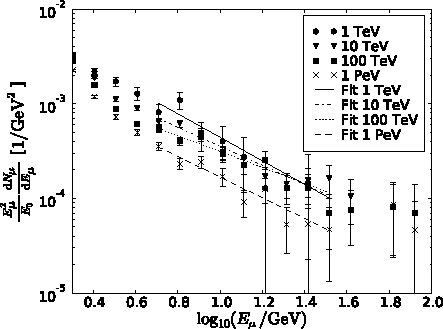
\includegraphics[width=0.8\textwidth]{./images/muon_flux_hadronic_shower.pdf}
    \caption{Differential muon flux for several injected hadronic energies. \cite{Panknin09ICRC}}
    \label{fig:mu_flux_hadr_shower}
\end{figure}
